\documentclass{standalone}
\usepackage{tikz}
\usepackage{ctex,siunitx}
\usepackage{tkz-euclide}
\usepackage{amsmath}
\usetikzlibrary{patterns, calc}
\usetikzlibrary {decorations.pathmorphing, decorations.pathreplacing, decorations.shapes,}
\begin{document}
\small
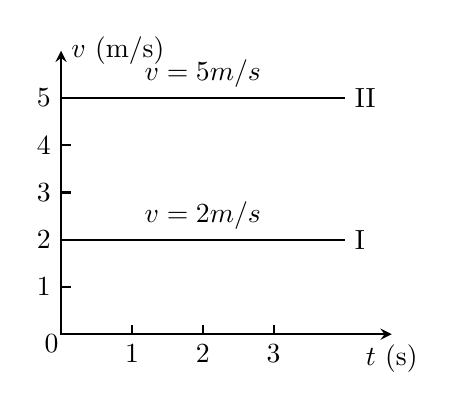
\begin{tikzpicture}[>=stealth, thick,scale=0.6]
  \draw [<->](0,6)node[right]{$v$ (\unit{m/s})}--(0,0)--(7,0)node[below]{$t$ (\unit{s})};
  \foreach \x in {1,2,3}
  {
      \draw(\x*1.5, 0) node[below]{$\x$} --(\x*1.5, .2);
  }
  \foreach \y in {1,2,3,...,5}
  {
      \draw(0,\y)node[left]{$\y$}--(.2, \y);
  }
  \node at (-.2,-.2){$0$};
  \draw (0,2)--node[above]{$v={2}{m/s}$}  (6,2)node[right]{I};
  \draw (0,5)--node[above]{$v={5}{m/s}$}  (6,5)node[right]{II};
\end{tikzpicture}
\end{document}